\chapter{Pré-traitement d'image\\ (Adrian)}

La bibliothèque SDL permet facilement de manipuler et charger des images, et
cela pour n'importe quel type de format (PNG, JPEG, BMP, \ldots). Il a donc
fallu dans un premier temps se familiariser avec cette bibliothèque à l'aide de
la documentation en ligne ainsi que du TP 3 de nos cours de programmation en C.

\section{Niveau de gris}

Transformer une image avec un niveau de gris est une opération basique de
traitement d'image. Pour cela, nous appliquons à chaque pixel la formule de la
luminance :

$L = 0.2126 \cdot R + 0.7152 \cdot G + 0.0722 \cdot B$

\begin{figure}[H]
    \centering
    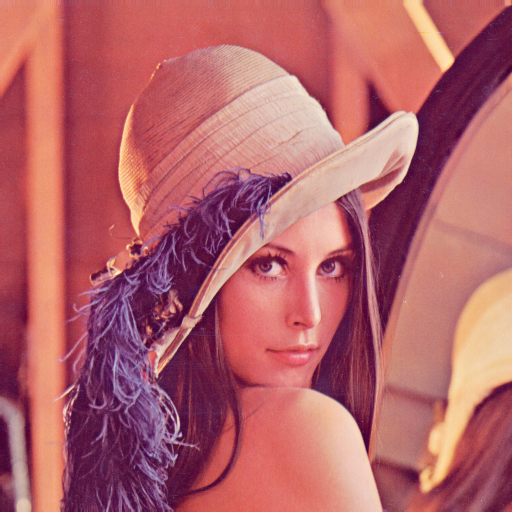
\includegraphics[width=0.3\textwidth]{lenna}
    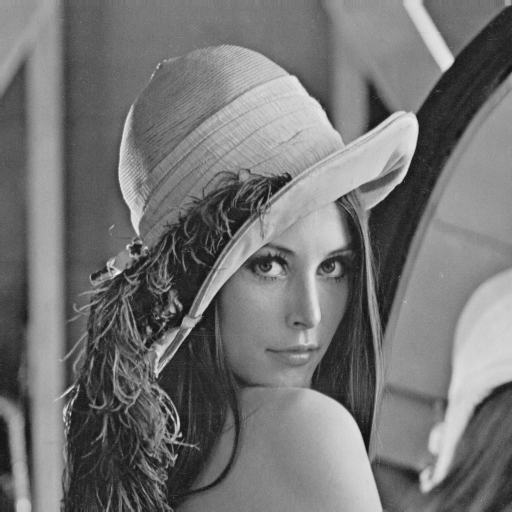
\includegraphics[width=0.3\textwidth]{lenna_gray}
    \caption{Niveau de gris}
\end{figure}

\section{Binarisation}

Pour binariser une image, la première étape est de choisir un seuil. Ce dernier
détermine si un pixel sera blanc ou noir (en fonction de s'il est inférieur ou
supérieur à ce seuil). Plusieurs méthodes existent pour choisir ce seuil, on
peut distinguer deux catégories :

\begin{itemize}
    \item \textbf{seuil fixe} : pour toutes les images un seuil est choisi pour
        décider si un pixel sera blanc ou noir.
    \item \textbf{seuil automatique} : chaque image est analysée pour déterminer
        un seuil adapté à cette dernière.
\end{itemize}

Sélectionner un seuil fixe est une solution facile à mettre en place mais peut
donner des résultats très variés en fonction de la qualité de l'image, de sa
luminosité ou encore des contrastes.

\begin{figure}[H]
    \centering
    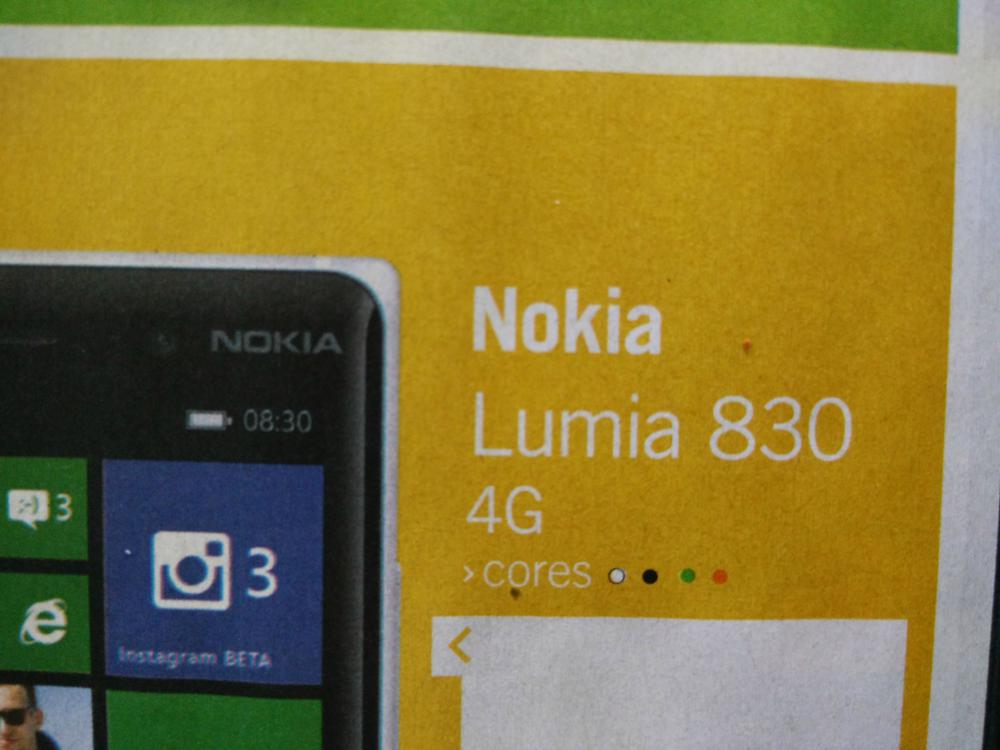
\includegraphics[width=0.4\textwidth]{fixed_threshold_00}
    \caption{Image originale en couleur}
\end{figure}

\begin{figure}[H]
    \centering
    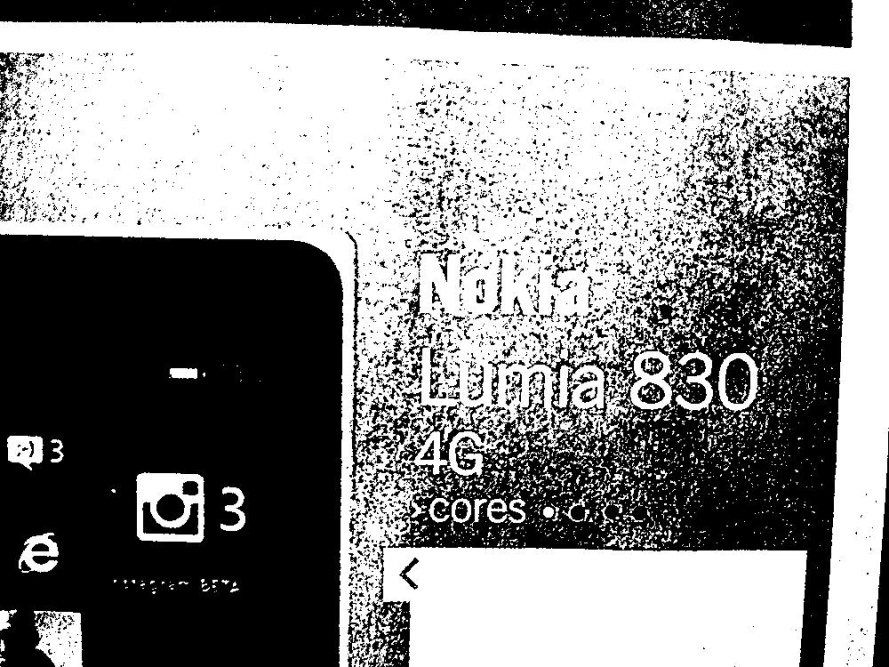
\includegraphics[width=0.4\textwidth]{fixed_threshold_01}
    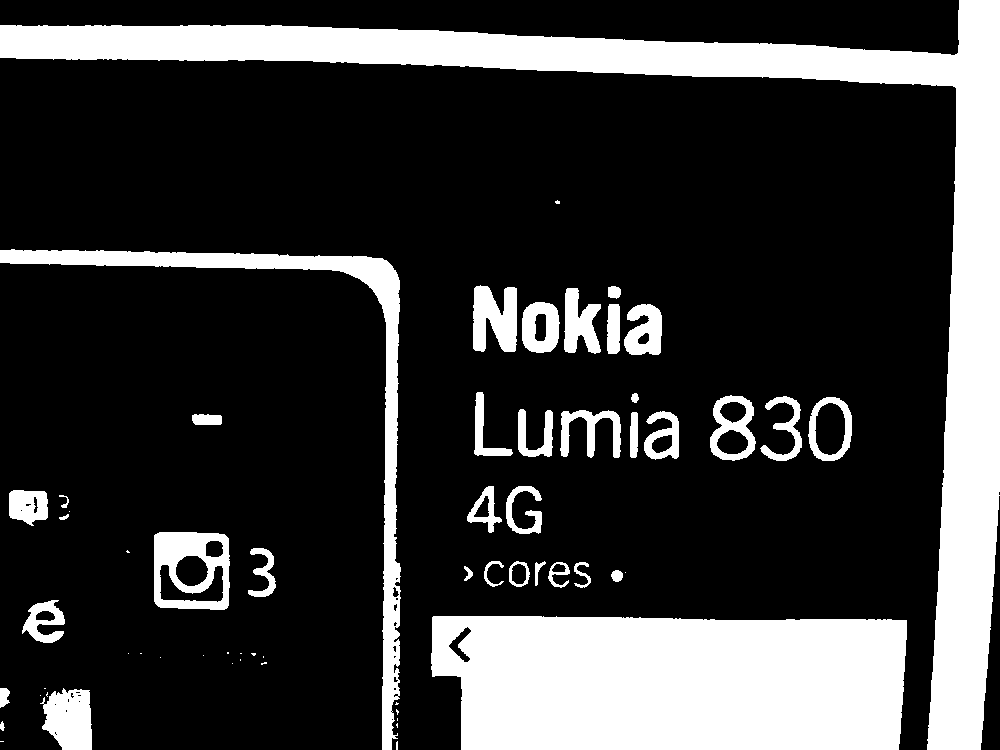
\includegraphics[width=0.4\textwidth]{fixed_threshold_02}
    \caption{Différents résultats à seuils fixes}
\end{figure}

\newpage

Nous avons donc opté pour l'option du seuil automatique. Encore une fois il y a
de nombreux algorithmes pour implémenter une telle fonctionnalité, celui retenu
est la \textbf{méthode d'Otsu}. L'idée derrière cet algorithme est de construire
un histogramme pour analyser la distribution des intensités de gris de l'image,
puis de calculer un seuil optimal distinguant le premier plan et l'arrière-plan.

\begin{figure}[H]
    \centering
    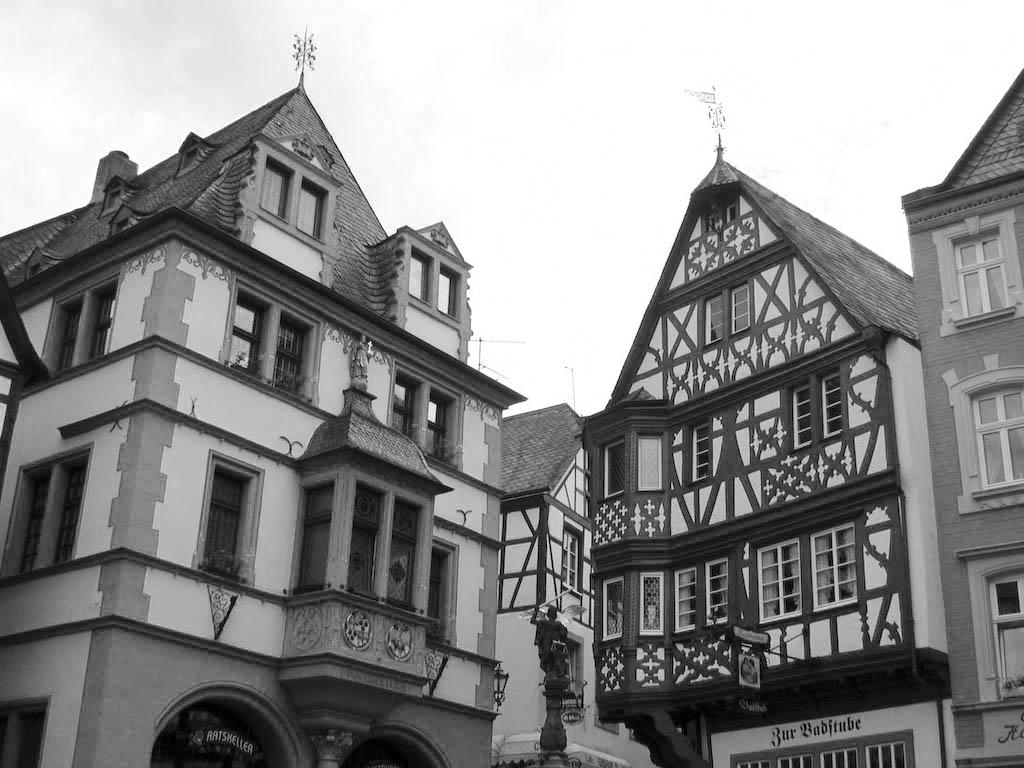
\includegraphics[width=0.45\textwidth]{houses}
    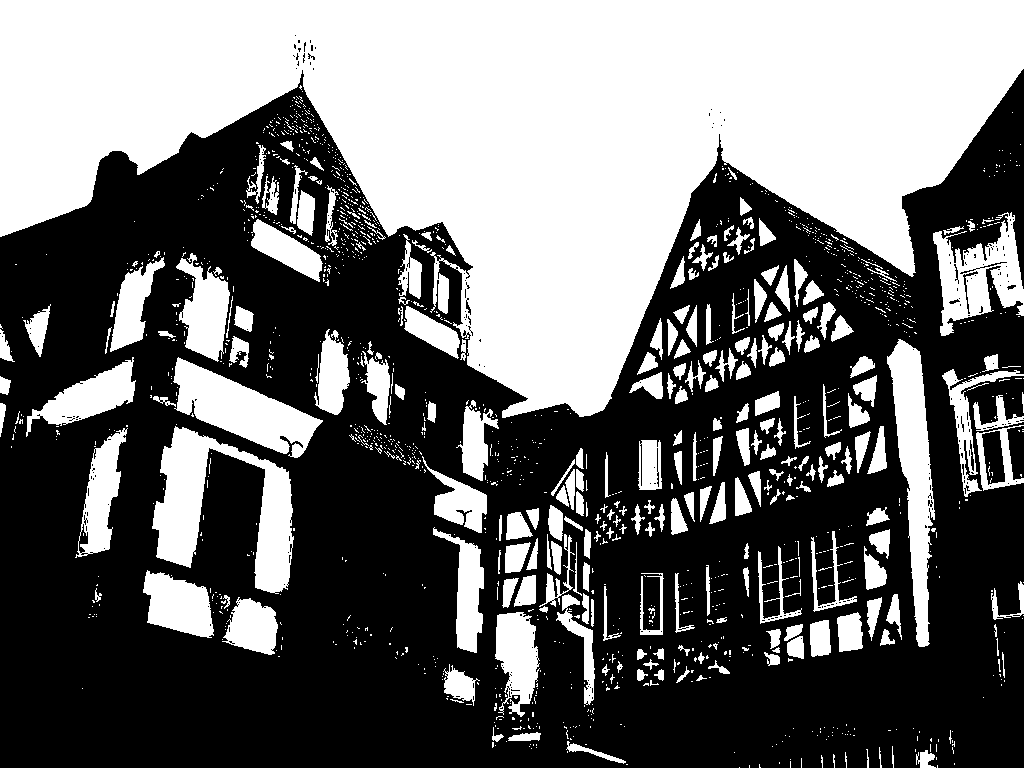
\includegraphics[width=0.45\textwidth]{houses_binarize}
    \caption{Binarisation à seuil automatique}
\end{figure}
